\documentclass{beamer}
\usepackage{lsfolien}
\usepackage[english]{babel}

\myfootline{Sustainability, Environment, Management -- Summer Term
  2022}{Hans-Gert Gr\"abe}

\title{On the Notion of a Resource\vskip1em}

\subtitle{Research Seminar in the Module 10-202-2312\\ for Master Computer
  Science}

\author{Prof. Dr. Hans-Gert Gräbe\\
\url{http://www.informatik.uni-leipzig.de/~graebe}}

\date{April 2022}
\begin{document}

{\setbeamertemplate{footline}{}
\begin{frame}
  \titlepage
\end{frame}}

\begin{frame}{Systems and Problem Solving}

The concept of system is a basic mental tool for delimiting and reducing
problems to their essentials.

Such focussing and contextualisation is the prerequisite for further planful
proceeding according to Darrell Mann: 
\begin{itemize}
\item for modelling the problematic situation ("Define"), 
\item for selection of suitable solution tools ("Select"), 
\item for generation of solution proposals ("Generate") and 
\item the assessment and selection of suitable solutions ("Evaluate").
\end{itemize}

D. Mann stops at this mental stage in his book, which of course must still be
followed by the implementation of the solution -- "it is not only about
interpreting the world differently, it is a matter of changing it" (Marx).
\end{frame}

\begin{frame}{The TRIZ Way of Thinking}
\small
  \begin{center}
  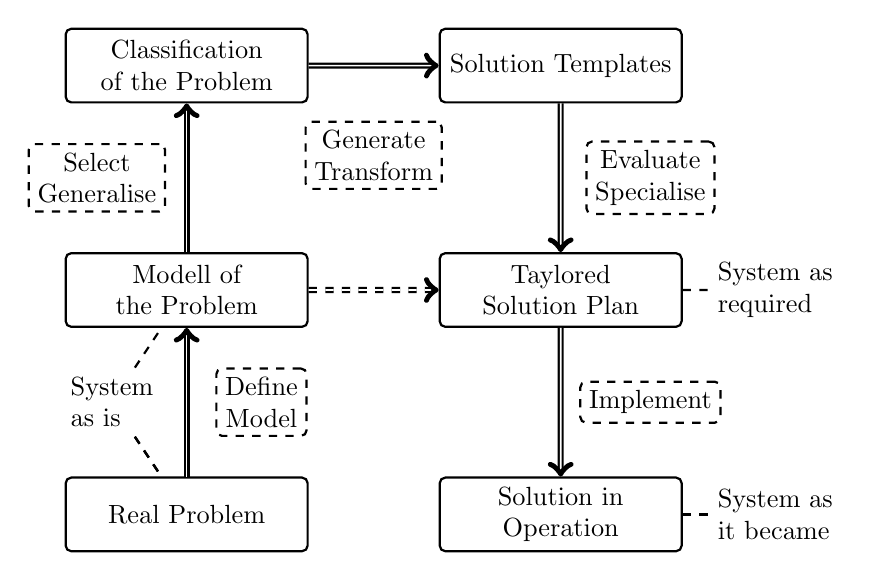
\begin{tikzpicture}[scale=.95,transform shape,
      textbox/.style={draw, text width=3cm, minimum height=2.8em,
        align=center},
      ovalbox/.style={draw, dashed, align=center},
      %>={Triangle[length=0pt 6,width=0pt 5]},
      rounded corners=2pt,line width=.8pt]

    \node[text width=1.1cm] at (-1,1.5) (A0) {System\\ as is};
    \node[textbox] at (0,0) (A1) {Real Problem};
    \node[ovalbox] at (1,1.5) {Define\\ Model}; 
    \node[textbox] at (0,3) (A2) {Modell of the Problem};
    \node[ovalbox] at (-1.2,4.5) {Select\\ Generalise}; 
    \node[textbox] at (0,6) (A3) {Classification of the Problem};
    \node[ovalbox] at (2.5,4.8) {Generate\\ Transform}; 
    \node[textbox] at (5,6) (B3) {Solution Templates};
    \node[ovalbox] at (6.2,4.5) {Evaluate\\ Specialise}; 
    \node[textbox] at (5,3) (B2) {Taylored\\ Solution Plan};
    \node[ovalbox] at (6.2,1.5) {Implement}; 
    \node[textbox] at (5,0) (B1) {Solution in Operation};
    \node[text width=1.8cm] at (8,3) (C2) {System as\\ required};
    \node[text width=1.8cm] at (8,0) (C1) {System as\\ it became};

    \draw[-,dashed] (A0) -- (A1);
    \draw[-,dashed] (A0) -- (A2);
    \draw[-,dashed] (B1) -- (C1);
    \draw[-,dashed] (B2) -- (C2);
    \draw[-,dashed] (A0) -- (A1);
    \draw[-,dashed] (A0) -- (A1);
    
    \draw[double,->] (A1) -- (A2) ;
    \draw[double,->] (A2) -- (A3) ;
    \draw[double,->] (A3) -- (B3) ;
    \draw[double,->,dashed] (A2) -- (B2) ;
    \draw[double,->] (B3) -- (B2) ;
    \draw[double,->] (B2) -- (B1) ;
\end{tikzpicture}
\end{center}
\end{frame}

\begin{frame}{Define}

This first step in Darrell Mann's approach starts with the delineation of an
appropriate systemic context for the study of the problem.
  \begin{itemize}
  \item Delimitation of the system externally against a "living" context as
    \emph{environment}. 
  \item Delineate the system internally -- delineate \emph{components} that
    either already exist (as \emph{artefacts} or as \emph{services}, i.e. also
    "belong to the environment") or are available at the time of assembling
    and operating the system.
  \end{itemize}

This allows concentration on the \emph{internal view} and planning of a
\emph{functional solution} to the problem.
\end{frame}

\begin{frame}{TRIZ Concept of the Ideal Machine}

In the TRIZ methodology \emph{functional} properties as "usefulness for
others" are in the foreground.

The terms \emph{usefulness} and \emph{harmfulness} play an important role in
TRIZ alongside the objectives of profitability and efficiency as
socio-cultural guiding principles.

With the concepts of \emph{Ideality} and \emph{Ideal Final Result} a mental
construct of anticipation of the functional properties of a system stands at
the beginning of its genesis.
\begin{block}{Koltze/Souchkov, p. 40}
  The ideal machine is a solution in which the maximum utility is achieved but
  the machine itself does not exist. 
\end{block}
\end{frame}

\begin{frame}{TRIZ Concept of the Ideal Machine}

The ideal machine is therefore \emph{pure functionality} without any
resource-related underpinning.

Nonetheless, that fictitious idea is central to TRIZ, for it develops a strong
orientation towards the intended usefulness and thus has a socio-cultural
guiding effect.

\emph{Machine} here stands very generally for "potentially working solution"
and hence applies also to problem solving in socio-technical systems as
organisations.
\end{frame}

\begin{frame}{Select, Generate, Evaluate}\small

Here Darrell Mann deviates somewhat from my scheme.

My „Generalise“ is rather part of „Define“ but not directed towards modelling
of the given problem, but at finding a \emph{working conceptual
  generalisation}.

„Select“ appropriate tools requires or is interwoven with finding this working
conceptual generalisation.

„Generate“ much depends on a good choice of tools and thus of a working
conceptual generalisation.  Hence the demarcation of the transformation on the
higher level of abstraction is slightly different.  

This also applies to „Specialise“. It is more than mere „Evaluation“ since it
comprises to taylor a general solution template to the given situation.

In both versions the process ends with a \emph{plan} for the implementation of
the solution.

\end{frame}

\begin{frame}{Implement}

This phase does not occur in Darrell Mann's work (and in TRIZ in general) in
such a clear way as it does, for example, in Design Thinking.

But the DT methodological approach is different: the methodological focus is
rather on the multiple rapid (agile) passing through the feedback cycle
between real problem and possible solutions instead of precise planning.

\end{frame}

\begin{frame}{Implement}

Implement in (or after) TRIZ means: 
\begin{itemize}
\item Machine must be "built".
\item Machine must be "deployed" at the given location and "come to life".
\item To do this, the \emph{operating conditions} (import and export) must be
  provided.
\item Which resources are needed (input) and which are made available (output). 
\end{itemize}
\vfill

What are resources in TRIZ? 
\vfill
\end{frame}

\begin{frame}{On the Notion of Resources in TRIZ}

\begin{block}{ARIZ-85C:}
  „Substance Field Resources are substances and fields that are already
  available or are (easily) obtainable according to the conditions of the
  task“.
\end{block}
  
Wessner lists a whole variety of concepts of resources proposed by different
TRIZ schools.  The spectrum ranges from 
\begin{itemize}
\item "a means that can be used to solve a problem" (Souchkov) 
\item to "anything in or around the system that is not being used to its
  maximum potential" (Mann, Salamatov)
\item to the notion of resource as source of a problem itself: "a problem
  always arises, if a needed resource is not present" (Orlov).
\end{itemize}

\end{frame}

\begin{frame}{On the Notion of Resources in TRIZ}\small

In (Koltze/Souchkov, p. 51) a resource is understood as "a means, a tool to
carry out an action or to make a process take place" and equipment, money
funds, raw material, energy or even people (human resources) are mentioned as
examples of resources.\vspace*{-.5em}

Furthermore ressources there are classified according to\vspace*{-1em}
\begin{itemize}
\item \emph{value} (free, not expensive, expensive),
\item \emph{quality} (harmful, neutral, useful),
\item \emph{quantity} (unrestricted, sufficient, insufficient) and
\item \emph{readiness for use} (ready, to be modified, to be developed).
\end{itemize}\vspace*{-1em}

Specific \emph{qualitative} determinations of such "substances and fields" as
resources play almost no role.\vspace*{-.5em}

Qualitative determinations in the sense of the fulfilment of a
\emph{specification} are, however, essential in more complex technical
contexts in order to ensure the \emph{operation} of a specific functional
property, which is to be provided by a systemic context.

\end{frame}

\begin{frame}{What is the Problem?} 

The constructed thing (partial system) that has been taken out must be
(re)placed in the overall context.  But this context can be operated only as a
\emph{unified whole} that cannot be disassembled from an operational point of
view. The whole can only be operated in an assembled state, and this
requirement to be "assembled" does not end at any system boundary either.

It means putting the "dead" partial system (after appropriate preparation)
into a "living" (itself being systemically structured) environment and
"starting it to operate".

\emph{Preparation:} In component software, a distinction is made between
deploy, install and configure as well as an explicit signal to switch from
preparation to operating mode.

\end{frame}

\begin{frame}{What is the Problem?} 

This induces a \emph{further systemic development} of the "living" environment
as a systemic complex, i.e. \emph{the whole changes}.

This requirement later to operate the system must already be present in the
entire (mental) development process.

How does this throughput of substance, energy and information appear in the
TRIZ modelling process?

\end{frame}

\begin{frame}{Operating a Minimal Technical System} 

In the TRIZ notion of a \emph{minimal technical system}, a \emph{tool} acts on
an \emph{object} (workpiece) to be processed in order to transform it into a
\emph{useful product}.

\begin{center}
  \begin{tikzpicture}[scale=.7,transform shape,
      textbox/.style={draw, text width=3cm, minimum height=2.8em,
        align=center},
      >={Triangle[length=0pt 6,width=0pt 5]},
      rounded corners=2pt,line width=.8pt]

    \node[textbox,text width=2cm] at (0,0) (A1) {Tool};
    \node[textbox] at (5,0) (A2) {Processed Object\\ Workpiece};
    \node[textbox,fill=lightgray] at (5,2) (A3) {Useful\\ Product};
    
    \draw[->,line width=2pt,gray] (A1) -- (A2);
    \draw[->,line width=2pt,gray] (A2) -- (A3);
\end{tikzpicture}
\end{center}

The concept of the \emph{ideal system} considers the tool as a purely
functional property, the effect of which to intentionally change the state of
the workpiece to a useful product is achieved without any additional efforts
and any wear of the tool.

In other words, it is not the tool but the \emph{imaginaton of the tool} that
creates the required action in such an \emph{ideal machine}.
\vskip1em
\end{frame}

\begin{frame}{Operating a Complete Technical System} 

\begin{center}
  \begin{tikzpicture}[scale=.9,transform shape,
      textbox/.style={draw, text width=1.5cm, minimum height=2.8em,
        align=center},
      >={Triangle[length=0pt 6,width=0pt 5]},
      rounded corners=2pt,line width=.8pt]

    \node[textbox] at (0,0) (A1) {Energy Source};
    \node[textbox] at (2.5,0) (A2) {Engine};
    \node[textbox] at (5,0) (A3) {Trans\-mission};
    \node[textbox] at (7.5,0) (A4) {Tool};
    \node[textbox,text width=1.6cm] at (10,0) (A5) {Processed Object};
    \node[textbox] at (5,1.8) (A6) {Control};
    
    \draw[->,line width=2pt,gray] (A1) -- (A2);
    \draw[->,line width=2pt,gray] (A2) -- (A3);
    \draw[->,line width=2pt,gray] (A3) -- (A4);
    \draw[->,line width=2pt,gray] (A4) -- (A5);
    \draw[->,line width=2pt,gray] (A6) -| (A2);
    \draw[->,line width=2pt,gray] (A6) -- (A3);
    \draw[->,line width=2pt,gray] (A6) -| (A4);
\end{tikzpicture}
\end{center}

In the classical understanding of a \emph{complete technical system} 
\begin{itemize}
\item the energy throughput is centered on the tool, 
\item the throughput of substance transports the workpieces 
\item and the throughput of information is directed to the control of the
  action.
\end{itemize}
Thus, in any case, the concept of a resource is understood as "means that can
be used to solve a problem."
\vskip1em

\end{frame}

\begin{frame}{Resources, Tools and State Changes} 

The understanding of the relationship of action conveyed here is asymmetrical.

An active tool has a state-changing effect on a passive workpiece, while
retaining its own functionality and -- ideally -- without undergoing a state
change itself.

In \emph{substance-field models} this understanding is replaced by a
more symmetrical model of a field-mediated action between two substances.

\begin{center}
    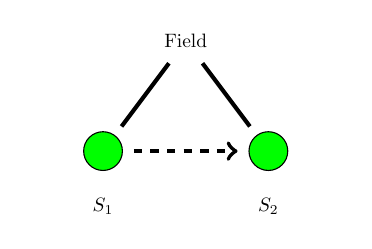
\begin{tikzpicture}[scale=.7,transform shape,
        pfeil/.style={shorten <=4pt, shorten >=4pt, line width=1.5pt},
        mytext/.style={text width=2.5cm,align=center}]
    \node[draw,fill=green,minimum size=2em] at (0,0) [circle] (A0) {};
    \node[draw,fill=green,minimum size=2em] at (3,0) [circle] (A1) {};
    \node at (1.5,2) [rectangle] (A2) {Field};
    \node[mytext,below of = A0] {$S_1$};
    \node[mytext,below of = A1] {$S_2$};
    \draw[pfeil,->,dashed] (A0)--(A1) ;
    \draw[pfeil,-] (A0)--(A2) ;
    \draw[pfeil,-] (A2)--(A1) ;
    \end{tikzpicture}
\end{center}

\end{frame}

\begin{frame}{Resources, Tools and State Changes} 

At the same time, in the systemic abstraction, the materiality of the
\emph{tool} is pushed back further in favour of the concept of \emph{action}
and a component concept is prepared as proposed by C. Szyperski for Component
Software.

There, \emph{components} are basically conceptualised as \emph{stateless} with
all the resulting consequences. In contrast to this \emph{objects} are
conceptualised as state-bearing units of instantiation to maintain a certain
standardisation of workpieces required for a repeated application of a
function within a production process.

\end{frame}

\begin{frame}{Resources, Tools and State Changes}

A similar idea comes through when Souchkov describes the two goals of
\emph{Resource Analysis} as essential component of TRIZ:
\begin{itemize}
\item Analysis of the resources that are to be \emph{treated or consumed} in
  the course of a process,
\item and analysis of the resources that can be \emph{used} to carry out the
  process or to solve the problem,
\end{itemize}
i.e., he distinguishes resources of the first kind, which undergo
state-changing transformations as \emph{workpieces} and resources of the
second kind, which are used as tools to \emph{mediate} these state changes.

\end{frame}

\begin{frame}{Operation and Maintenance of Technical Systems} 

Such a notion also corresponds well with the widespread organisation of
production processes, where a distinction is made between operating and
maintenance mode.

In the operating mode, the focus is on the functional properties of the tool,
while in the maintenance mode its material properties are focused.

As an independent technical system in a narrower sense, only the
operating mode is modelled as the target of a "problem solution".

The maintenance mode is part of the supersystem, which is concerned with the
\emph{reproduction} of the tools as \emph{resources} used in the operating
mode.

\end{frame}

\begin{frame}{Operation and Maintenance of Technical Systems} 

In the (classical) operating mode the focus is on the use of tools and
the material throughput of workpieces, which are thereby transformed into
useful products, in many cases \emph{technical artefacts}, which are either
further processed as semi-finished products in a following technical system or
enter into such contexts as tools themselves.

In both cases the useful product is a \emph{resource} for further systemic
processes.

But TRIZ is not (primarily) about system analysis but about \emph{problem
  solving} and the design of viable technical systems in a \emph{systemic
  development} \textbf{process}.

\end{frame}

\begin{frame}{Systemic Development and Problem Solving}
  
Souchkov clarifies the role of \emph{Resource Analysis} in such a process:
\begin{quote}\small
  A technical system has different resources at its disposal for the
  completion of its function. A function can only be completed using suitable
  resources. Resources are therefore elementary building blocks of a problem
  solution. The skilful use of resources distinguishes an efficient from an
  inefficient system.
\end{quote}

The question of systemic operating conditions is thus reversed -- it is not
about what conditions are \emph{required} for the operation of a particular
system, but what kind of system under \emph{given} operating conditions
promises an efficient problem solution.

The focus thus shifts from the operating conditions of an existing system to
the question of a systemic development and co-evolution in a given context.

\end{frame}

\begin{frame}{The World of Technical Systems}

The operational demand of a technical system is formulated in the form of
\emph{specifications} as requirements to the "environment", which must be
fulfilled for the \emph{operation} of the system. Thus the "reduction to the
essentials" that characterises the systemic approach is only a
\emph{conditional} mind game that presupposes a sufficiently powerful
\emph{environment} as given, in which the necessary \emph{resources} can be
found to fulfil the operating conditions.

Sommerville emphasises the importance of such interface specification for the
development of software systems that "need to interoperate with other systems
that have already been developed and installed in the environment."

\end{frame}

\begin{frame}{Components as Resources and Component Models}

The same perspective is significant when large systems are to be created in a
cooperative development process and for this a decomposition into subsystems
is required that are to be developed independently of each other.

This development process in turn requires a more extensive socio-technical
infrastructure with
\begin{enumerate}
\item \emph{independent components} that can be fully configured via their
  interfaces,
\item \emph{standards for components} that simplify their integration, 
\item a \emph{middleware}, which supports the component integration with
  software
\item and a \emph{development process} that is designed for component-based
  software engineering.
\end{enumerate}

\end{frame}

\begin{frame}{Components as Resources and Component Models}

Components are thus conceptually integrated into an overarching
\emph{component model}, which essentially ensures the technical
interoperability of different components beyond concrete interface
specifications and thus forms a moment of unity in the diversity of the
components.

However, this unity extends not only to the model, but also to the operating
conditions of the components (as functional property of the middleware) as
well as to their socio-technical development conditions (as a partial
formalisation of the development process).

This frame constitutes as \emph{component framework} (Szyperski) a
socio-technical supersystem as an "environment" of components that were
created according to the specifications of that component model.
  
\end{frame}

\begin{frame}{The World of Component Models}

Szyperski, for his part, analyses this diversity of compatibilities and
incompatibilities of different component models and identifies different
levels of abstraction for the reuse of concepts that go beyond the use of
prefabricated components.

In his 20-year-old book he already emphasises
\begin{quote}\small
  the growing importance of component deployment, and the relationship between
  components and services, the distinction of deployable components (or just
  components) from deployed components (and, where important, the latter again
  from installed components). Component instances are always the result of
  instantiating an installed component -- even if installed on the fly.
  Services are different from components in that they require a service
  provider.  
\end{quote}
  
\end{frame}

\begin{frame}{Functional and Attributive Properties}

Szyperski shows that the component approach is an approach of reuse that is
not limited to the (possibly modified) abstract reuse of the technical
functionality of a problem solution, but always reuses components together
with their operating conditions as \emph{services} and thus not detached from
their environment.

For this, Shchedrovitsky's distinction between functional and attributive
properties as well as the distinction between the notions of \emph{part} and
\emph{element} are essential.  
\begin{quote}\small
  {\bf Elements} are what a unity is made up of, so an element is a part
  inside the whole, which functions inside the unity, without as it were being
  torn out of it. A simple body, a {\bf part}, is what we have when everything
  has been disassembled and is laid out separately. But elements only exist
  within the structure of {\bf connections}. So an element implies two
  principally different types of properties: its properties as material, and
  its functional property derived from connections.
\end{quote}
\end{frame}

\begin{frame}{Functional and Attributive Properties}
\begin{quote}\small
  In other words, an element is not a part. A part exists when we mechanically
  divide something up, so that each part exists on its own as a simple body.
  An element is what exists in connections within the structure of the whole
  and functions there. [\ldots]\vskip1em

  {\bf Functional properties} belong to an element to the extent that it
  belongs to the structure with connections, while other properties belong to
  the element itself. If I take out this piece of material, it preserves its
  {\bf attributive properties}. They do not depend on whether I take it out of
  the system or put it into the system. But functional properties depend on
  whether or not there are connections. They belong to the element, but they
  are created by a connection; they are brought to the element by connections.
\end{quote}

\end{frame}

\begin{frame}{Filling the Places with Content}
The terms \emph{part}, \emph{element}, \emph{connection} describe the
\emph{structure} of the place in the system itself, where the connection of
the "dead" system with the "living" world must be carried out in order to
bring the system itself to life.

In the further system genesis, this conceptual frame has to be filled with
suitable resources. How conceptualise this "filling“, the combination of the
functional properties at the "connections" with resources to an almost
ideal machine?

To describe this composition process ("components are for composition" --
Szyperski) Shchedrovitsky distinguishes the concepts \emph{place} and
\emph{content}.

\end{frame}

\begin{frame}{Filling the Places with Content}
\begin{quote}\small
  Doing that, we introduce the concepts of place and content. An {\bf element}
  is a unity of a place and its content – the unity of a functional place, or
  a place in the structure, and what fills this place.\vskip1em

  A {\bf place} is something that possesses functional properties. If we take
  away the content, take it out of the structure, the place will remain in the
  structure, held there by {\bf connections}. The place bears the totality of
  functional properties.\vskip1em

  The {\bf content} by contrast is something that has attributive functions.
  Attributive functions are those that are retained by the content of a place,
  when this content is taken out of the given structure. We never know whether
  these are its properties from another system or not. Now we might take
  something out as content, but it is in fact tied to another system, which,
  as it were, extends through this place. 
\end{quote}
\end{frame}

\begin{frame}{Filling the Places with Content}
The search for resources is constitutive for the process of confinement in the
course of the genesis of the system that is to be developed from the pure
functionality of the ideal machine.  This corresponds to Altshuller's first
law of systemic development.
\begin{block}{Altshuller's Law of the Completeness of the Parts of a System}
  The necessary condition for the viability of a technical system is the
  existence of the main parts of the system {\bf and} their minimal
  functionality (i.e. viability -- HGG).
\end{block}
\vfill

However, the thing viewed with the magnifying glass as a connection of place
and content remains a "dead body", because "a living being has no parts"
(Shchedrovitsky).

\end{frame}

\begin{frame}{Connecting Systems. The Operational Dimension}
It is of little use to dissect a living frog in order to see how place and
content are to be combined, since you cannot study the blood flow in its veins
this way.

It is not enough that the plug fits into the socket, the socket must also
"have power in it". 

Beyond the connection of place and content an operational process dimension is
essential for a living system.  Shchedrovitsky develops that as a \emph{second
  concept of a system}.  This cannot be explained here.

We are dealing with a typical phenomenon of a modern society, in which the
electricity comes from the socket and the milk from the shop.  The division of
labour in such a modern mode of production leads to the emergent phenomenon of
social unity and stratification of the reproduction of infrastructural
conditions.

\end{frame}

\begin{frame}{Connecting Systems. The Operational Dimension}

The existence, reliability and robustness (resilience) of such an
infrastructure has a significant influence on the way people organise their
daily lives.

With the insight into ever more complex interrelationships, a concept of
resources as "anything in or around the system that is not being used to its
maximum potential" (Mann, Salamatov), which focuses on the \emph{exploitation}
of resources, becomes increasingly counterproductive and has to be replaced by
a concept of resources with socio-culturally institutionalised forms of
\emph{resource management} at its center.

\end{frame}

\begin{frame}{The Concept of a Resource and the Mode of Production}

\begin{block}{Thesis:}
  The concept of resource exploitation is a characteristic feature of all
  existing so far forms of a capitalist mode of production.
\end{block}

It manifests a fundamental contradiction of socio-cultural development:
without such exploitation we would not have reached the current state of
technology, but at the same time we undermine our own conditions of existence.

My historical optimism says that it is nevertheless precisely these means of
increasing conceptual penetration of ever increasingly complex
interrelationships by which this trend can be stopped and eventually reversed.

\end{frame}

\begin{frame}{The Global Scope of Local Action}
The formulated contradiction is of a global, planetary dimension that cannot
be solved by the regional disposition of individual power groups over
exploitable resources.  The division of the world into spheres of influence
thus becomes obsolete insofar as in each of these spheres of influence, the
transition to a different form of using resources must be organised to avoid a
global environmental collapse of the resources used by mankind in the long
run.

TRIZ systemic evolution trends of increasing coordination, controllability and
dynamisation refer not only to \emph{system-internal development lines}, but
also to the coordination \emph{between} systems which are operated by
independent third parties.

Qualifying the infrastructural framework, for example, of the power supply
system as "supersystem" does not take into account the relations of
\emph{mutual interdependency} in such a modern industrial mode of production.

\end{frame}

\end{document}
